\chapter{Измерения, приближения и практические расчёты}\label{chap:exam-measurements}\markright{Глава 4}
\section{Величины и единицы}
\begin{definition}\term{Физическая величина} (\emph{physical quantity}) описывает измеримое свойство; её числовое значение зависит от единицы. Например, одна длина может быть записана как \(1{,}5\) м или \(150\) см. \par\term{Размерность} (\emph{dimension}) указывает тип величины: длина, время, площадь, скорость.\end{definition}
При переводе единиц изменяется число, а величина сохраняется. Из \(1\text{ м}=100\text{ см}\) следует \(1\text{ м}^2=10000\text{ см}^2\), \(1\text{ м}^3=10^6\text{ см}^3\). Литр равен кубическому дециметру, гектар --- \(10000\text{ м}^2\). Для скорости \(1\text{ м/с}=3{,}6\text{ км/ч}\). Время \(1{,}5\) часа означает час и тридцать минут, а не час пятьдесят минут.
\begin{example}Комната имеет размеры \(3{,}2\) м и \(450\) см. Приводим длины к метрам: \(450\text{ см}=4{,}5\text{ м}\). Площадь \(3{,}2\cdot4{,}5=14{,}4\text{ м}^2\). Для квадратной плитки со стороной \(40\) см площадь одной плитки \(0{,}16\text{ м}^2\); по отношению площадей получается нижняя оценка \(\frac{14{,}4}{0{,}16}=90\) плиток. Реальная раскладка с учётом размеров и обрезки может потребовать большего количества.\end{example}
\section{Округление и направленное округление}
\begin{definition}\term{Округление до разряда} (\emph{rounding to a place value}) заменяет число ближайшим кратным единицы этого разряда. При точном попадании посередине в школьных вычислениях увеличивают модуль оставляемой части: \(2{,}35\mapsto2{,}4\), \(-2{,}35\mapsto-2{,}4\) при округлении до десятых.\end{definition}
Смотрим на первую отбрасываемую цифру: \(0,1,2,3,4\) оставляют предыдущий разряд; \(5,6,7,8,9\) увеличивают его на единицу с переносом. Например, \(9{,}996\approx10{,}00\) до сотых. Последовательное округление через промежуточные разряды может дать другой результат: \(2{,}449\) сразу до десятых даёт \(2{,}4\), а через сотые --- \(2{,}5\). Округляй исходное число один раз в требуемом разряде.
\begin{definition}\term{Целая часть снизу} (\emph{floor}) \(\lfloor x\rfloor\) --- наибольшее целое, не превосходящее \(x\). \par\term{Целая часть сверху} (\emph{ceiling}) \(\lceil x\rceil\) --- наименьшее целое, не меньшее \(x\).\end{definition}
\begin{example}Для перевозки \(137\) человек в автобусах на \(48\) мест нужно \(\lceil\frac{137}{48}\rceil=3\) автобуса. Из \(137\) м ленты получатся \(\lfloor\frac{137}{48}\rfloor=2\) целых отрезка длиной \(48\) м. Одинаковое деление приводит к разному округлению из-за разных требований задачи. Для отрицательного числа \(\lfloor-1{,}2\rfloor=-2\), \(\lceil-1{,}2\rceil=-1\).\end{example}
\section{Абсолютная и относительная погрешность}
\begin{definition}\term{Абсолютная погрешность} (\emph{absolute error}) приближения \(\widetilde x\) к точному \(x\) равна \(|x-\widetilde x|\). \par\term{Относительная погрешность} (\emph{relative error}) при \(x\ne0\) равна \(\frac{|x-\widetilde x|}{|x|}\); для процентов её умножают на \(100\%\).\end{definition}
Запись \(x=\widetilde x\pm\Delta\) означает гарантированное включение \(\widetilde x-\Delta\le x\le\widetilde x+\Delta\), а не два возможных значения. Погрешность округления до шага \(h\) не превосходит \(\frac{h}{2}\). Не путай относительную погрешность относительно точного числа с отношением к приближённому числу: второе иногда используют как оценку, но это другая величина.
\begin{theorem}[Оценки ошибок суммы и произведения]
Если \(|x-a|\le\alpha\), \(|y-b|\le\beta\), то
\[
|(x+y)-(a+b)|\le\alpha+\beta,
\]
\[
|xy-ab|\le|a|\beta+|b|\alpha+\alpha\beta.
\]
\end{theorem}
\par\addvspace{2pt}\begin{lrbox}{\CatFlowBox}\begin{minipage}[t]{\linewidth}
\setlength{\parskip}{2pt}\setlength{\columnsep}{4.5mm}\setlength{\intextsep}{0pt}
\begin{wrapfigure}[11]{l}{54mm}
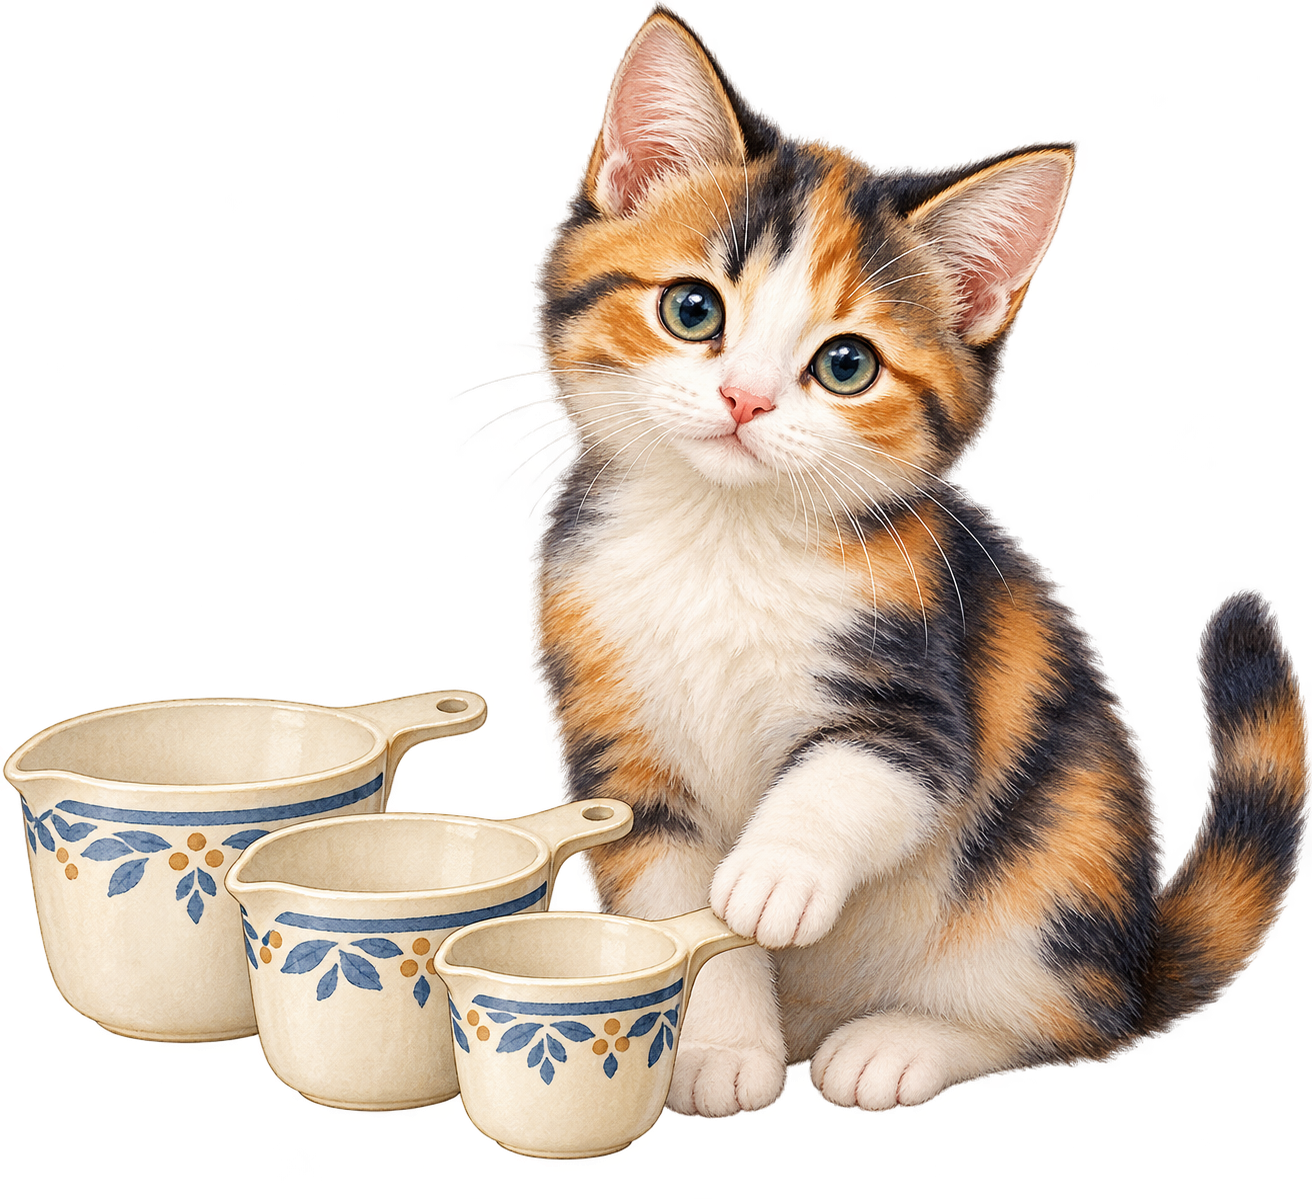
\includegraphics[width=54mm,height=58mm,keepaspectratio]{images/unique/art-197.png}
\label{catflow:197}
\end{wrapfigure}
\textit{Доказательство.} Для суммы применяем неравенство треугольника. Для произведения пишем \(x=a+u\), \(y=b+v\), где \(|u|\le\alpha\), \(|v|\le\beta\). Тогда \(xy-ab=av+bu+uv\); оцениваем каждое слагаемое по модулю.\hfill\(\blacksquare\)
\par\WFclear\end{minipage}\end{lrbox}%
\ifdim\dimexpr\ht\CatFlowBox+\dp\CatFlowBox\relax<58mm\dp\CatFlowBox=\dimexpr58mm-\ht\CatFlowBox\relax\fi%
\noindent\usebox{\CatFlowBox}\par\addvspace{2pt}

\begin{example}Длины прямоугольника равны \(3{,}0\pm0{,}1\) м и \(4{,}0\pm0{,}1\) м. Положительность сторон даёт точный гарантированный диапазон площади: \(2{,}9\cdot3{,}9\le S\le3{,}1\cdot4{,}1\), то есть \(11{,}31\le S\le12{,}71\). Симметричная оценка около \(12\) по теореме: \(|S-12|\le0{,}71\); она верна, хотя нижняя граница \(11{,}29\) менее точна.\end{example}
\section{Проценты, масштаб и чтение данных}
\begin{definition}\term{Процентный пункт} (\emph{percentage point}) --- единица разности двух величин, уже выраженных в процентах. Изменение доли с \(20\%\) до \(25\%\) равно \(5\) процентным пунктам и относительному росту на \(25\%\).\end{definition}
Масштаб \(1:m\) означает отношение длины на плане к реальной длине при одинаковых единицах. Площади относятся как \(1:m^2\), объёмы --- как \(1:m^3\). Для расхода \(c\) литров на \(100\) км на путь \(s\) км нужно \(\frac{cs}{100}\) литров. Если товары продаются упаковками, после расчёта количества нужно округление вверх.
\par\addvspace{2pt}\begin{lrbox}{\CatFlowBox}\begin{minipage}[t]{\linewidth}
\setlength{\parskip}{2pt}\setlength{\columnsep}{4.5mm}\setlength{\intextsep}{0pt}
\begin{wrapfigure}[11]{r}{54mm}
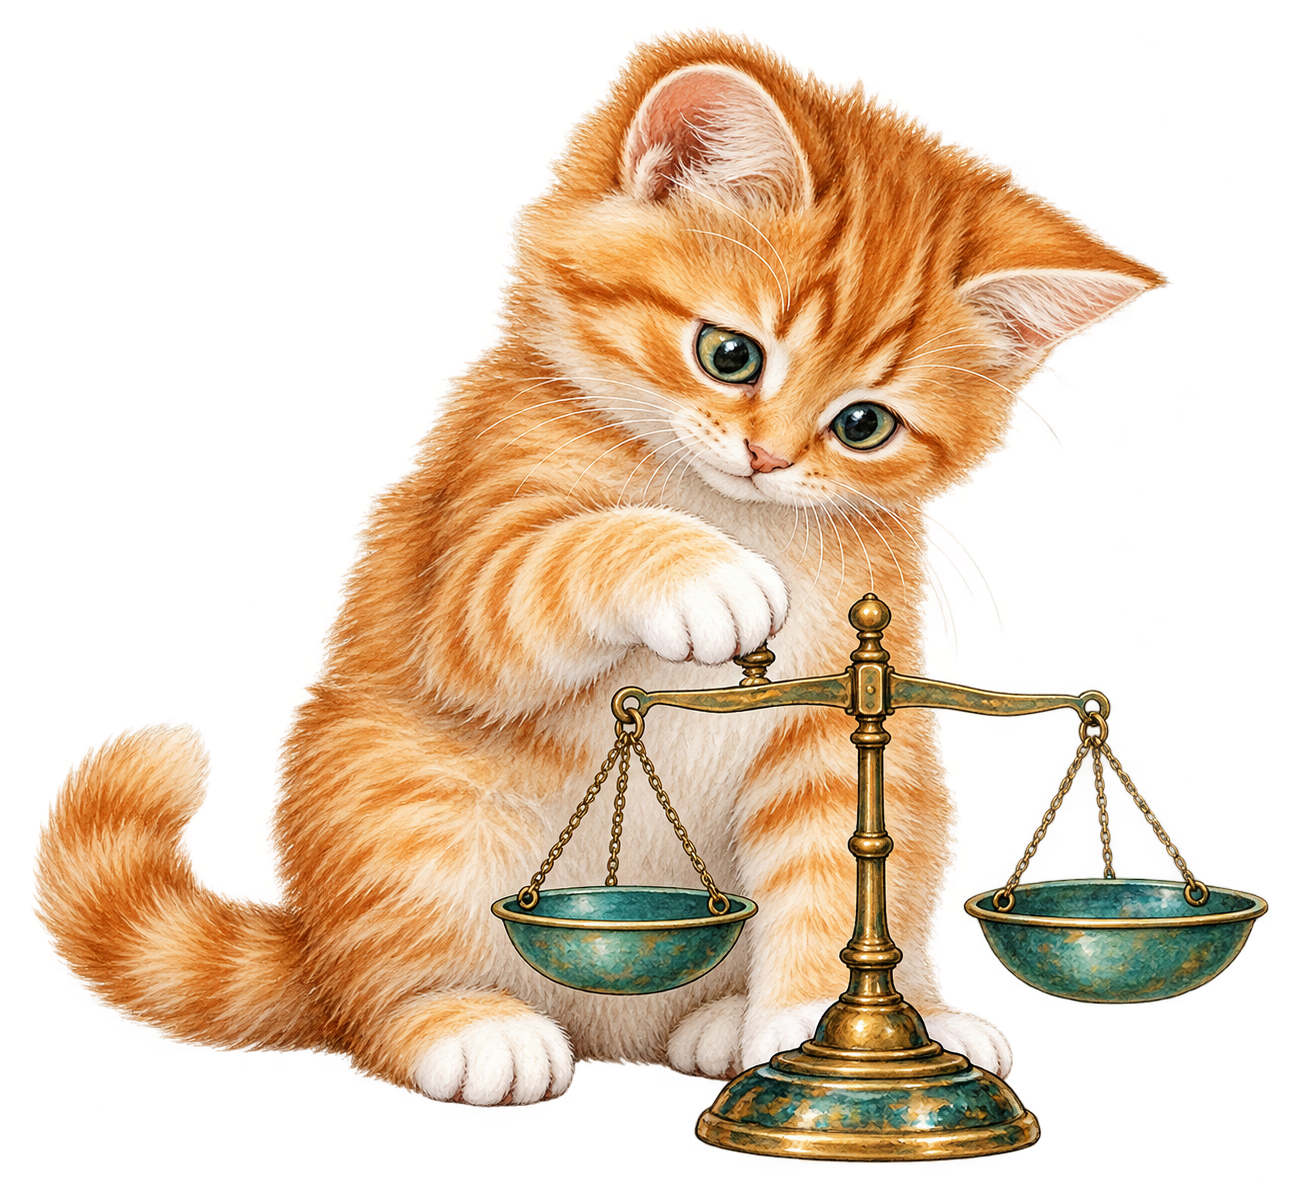
\includegraphics[width=54mm,height=58mm,keepaspectratio]{images/unique/art-194.png}
\label{catflow:194}
\end{wrapfigure}
Практическая задача начинается с определения величины, которую спрашивают. Подпись «тыс. рублей» меняет числовое значение в тысячу раз; площадь закрашенного участка на схеме не всегда совпадает с площадью всего участка. Сначала выпиши единицы и ограничения, затем переведи данные в одну систему. Когда в условии сказано, что покупать можно лишь целыми упаковками, ответ должен удовлетворять именно этому ограничению. Округление до ближайшего целого здесь может оставить часть работы невыполненной. Полезная последняя проверка состоит в подстановке выбранного количества в исходную ситуацию: помещаются ли люди, покрывается ли площадь, хватает ли денег. Так арифметический результат получает смысл ответа.
\par\WFclear\end{minipage}\end{lrbox}%
\ifdim\dimexpr\ht\CatFlowBox+\dp\CatFlowBox\relax<58mm\dp\CatFlowBox=\dimexpr58mm-\ht\CatFlowBox\relax\fi%
\noindent\usebox{\CatFlowBox}\par\addvspace{2pt}
\begin{example}На плане \(1:200\) прямоугольный участок имеет стороны \(3\) и \(4\) см. В действительности это \(6\) и \(8\) м, площадь \(48\text{ м}^2\). Если газон продаётся рулонами по \(2{,}5\text{ м}^2\), то при отсутствии потерь нужно \(\lceil\frac{48}{2{,}5}\rceil=20\) рулонов.\end{example}
\par\addvspace{2pt}\begin{lrbox}{\CatFlowBox}\begin{minipage}[t]{\linewidth}
\setlength{\parskip}{2pt}\setlength{\columnsep}{4.5mm}\setlength{\intextsep}{0pt}
\begin{wrapfigure}[9]{l}{54mm}
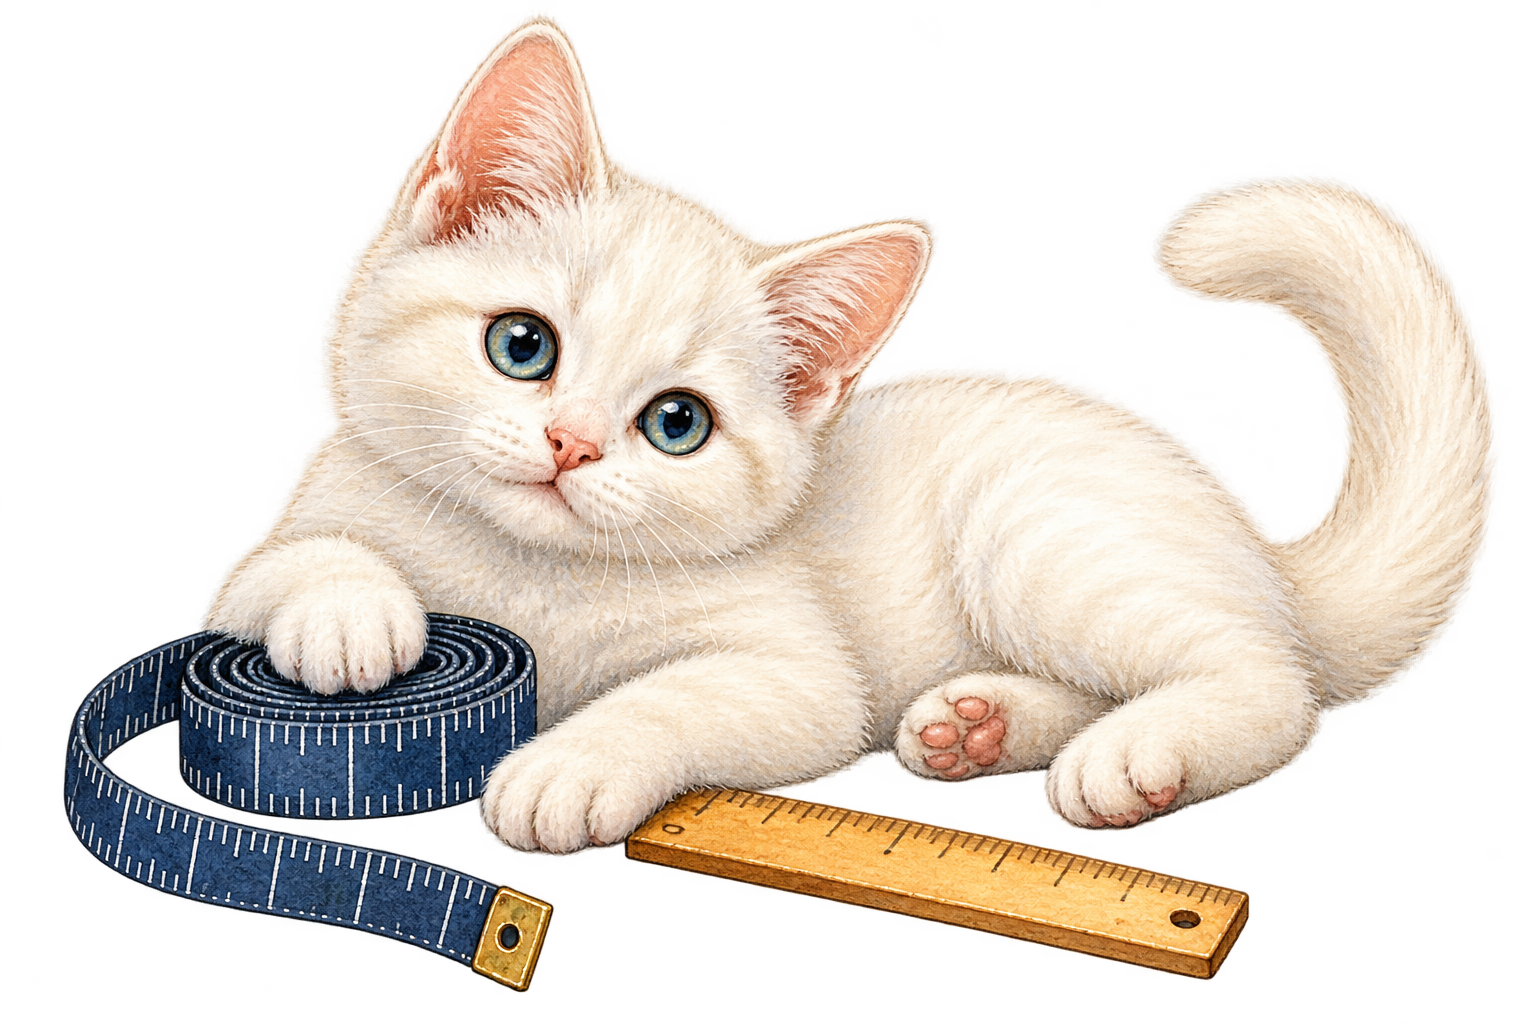
\includegraphics[width=54mm,height=58mm,keepaspectratio]{images/unique/art-195.png}
\label{catflow:195}
\end{wrapfigure}
При чтении таблицы нужно различать строку, столбец и единицу. На графике по горизонтальной оси часто откладывают время, по вертикальной --- накопленный объём, расстояние или температуру. Значение функции читают по высоте точки, изменение --- как разность высот, а среднюю скорость изменения --- как отношение изменения к длине временного промежутка. Ломаная между измерениями описывает принятую модель и сама по себе не доказывает, что между измерениями процесс был линейным. Для сравнения вариантов вычисляют одну и ту же итоговую величину при одинаковых условиях, учитывая фиксированную часть оплаты, ограничения тарифа и границы применимости формулы.
\par\WFclear\end{minipage}\end{lrbox}%
\ifdim\dimexpr\ht\CatFlowBox+\dp\CatFlowBox\relax<58mm\dp\CatFlowBox=\dimexpr58mm-\ht\CatFlowBox\relax\fi%
\noindent\usebox{\CatFlowBox}\par\addvspace{2pt}
\section{Прикидка и проверка размерности}
\begin{example}Для \(19{,}8\cdot5{,}1\) прикидка \(20\cdot5=100\) показывает порядок ответа; точное значение \(100{,}98\). Ответ \(1009{,}8\) подозрителен ещё до повторного умножения. Скорость \(\frac{s}{t}\) имеет размерность длина/время; формула \(s+t\) для скорости невозможна, если \(s\) --- путь, а \(t\) --- время.\end{example}
\par\addvspace{2pt}\begin{lrbox}{\CatFlowBox}\begin{minipage}[t]{\linewidth}
\setlength{\parskip}{2pt}\setlength{\columnsep}{4.5mm}\setlength{\intextsep}{0pt}
\begin{wrapfigure}[9]{r}{54mm}
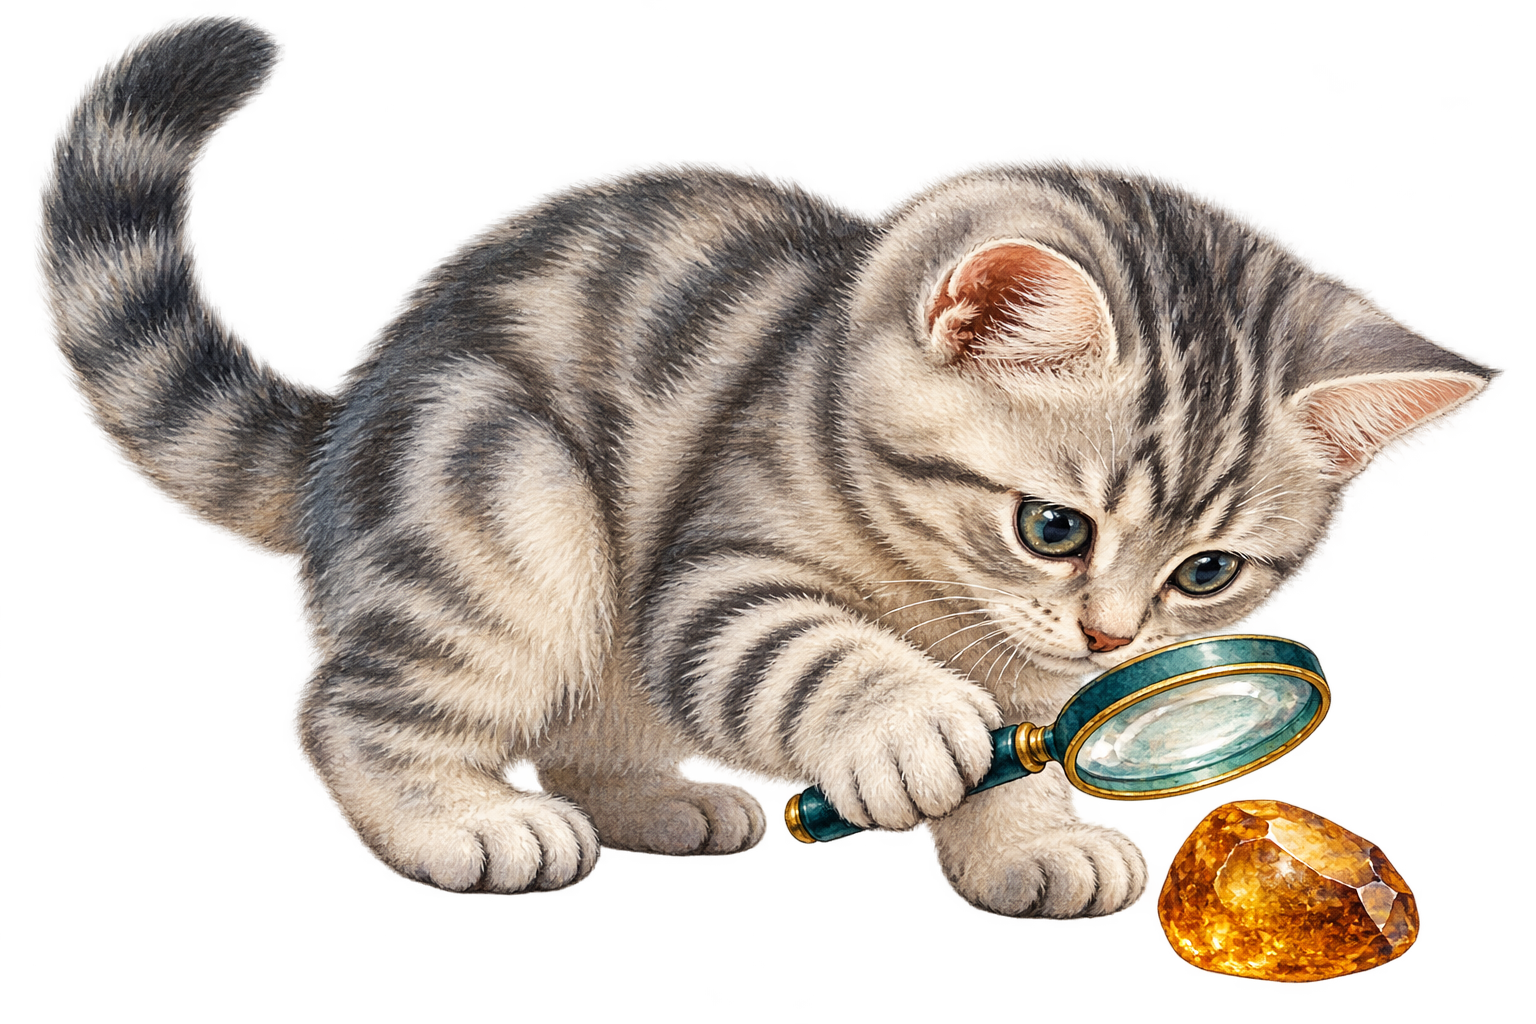
\includegraphics[width=54mm,height=58mm,keepaspectratio]{images/unique/art-196.png}
\label{catflow:196}
\end{wrapfigure}
В приближённых данных важно отделять точную информацию от результата измерения. Цена по тарифу, указанная в копейках, может быть точным условием модели, а длина, снятая с чертежа линейкой, обычно имеет допуск. Лишние цифры в результате деления не превращают неточные данные в точные. Если требуется гарантированный ответ, работай с границами интервала и учитывай монотонность выражения. Например, при неотрицательном числителе и положительном знаменателе нижняя оценка дроби получается из меньшего числителя и большего знаменателя. Для отрицательного числителя при увеличении положительного знаменателя дробь возрастает: знак числителя меняет зависимость от знаменателя. Если допустимый интервал знаменателя содержит ноль, такое правило без дополнительного разбора применять нельзя. Заверши решение проверкой того, что итоговое округление соответствует вопросу.
\par\WFclear\end{minipage}\end{lrbox}%
\ifdim\dimexpr\ht\CatFlowBox+\dp\CatFlowBox\relax<58mm\dp\CatFlowBox=\dimexpr58mm-\ht\CatFlowBox\relax\fi%
\noindent\usebox{\CatFlowBox}\par\addvspace{2pt}
\relax

\Needspace{7\baselineskip}\section*{Задачи}
\begingroup\setlength{\parskip}{1pt}
\noindent\begin{minipage}[t]{\linewidth}\textbf{4.1.} Переведи \(2{,}7\) км в метры, а \(360\) см в метры.\par\end{minipage}\par
\noindent\begin{minipage}[t]{\linewidth}\textbf{4.2.} Переведи \(0{,}08\text{ м}^2\) в квадратные сантиметры и \(750\) мл в литры.\par\end{minipage}\par
\noindent\begin{minipage}[t]{\linewidth}\textbf{4.3.} Вырази \(72\) км/ч в м/с, а \(15\) м/с в км/ч.\par\end{minipage}\par
\noindent\begin{minipage}[t]{\linewidth}\textbf{4.4.} Сколько минут в \(2{,}35\) часа?\par\end{minipage}\par
\noindent\begin{minipage}[t]{\linewidth}\textbf{4.5.} Округли \(7{,}8649\) до сотых и до десятых.\par\end{minipage}\par
\par\addvspace{2pt}\begin{lrbox}{\CatFlowBox}\begin{minipage}[t]{\linewidth}
\setlength{\parskip}{2pt}\setlength{\columnsep}{4.5mm}\setlength{\intextsep}{0pt}
\begin{wrapfigure}[11]{r}{54mm}

\includegraphics[width=54mm,height=58mm,keepaspectratio]{images/unique/art-198.png}
\label{catflow:198}
\end{wrapfigure}
\textbf{4.6.} Округли \(99{,}995\) до сотых по школьному правилу.\par

\textbf{4.7.} Найди \(\lfloor3{,}8\rfloor,\lceil3{,}8\rceil,\lfloor-3{,}8\rfloor,\lceil-3{,}8\rceil\).\par

\textbf{4.8.} Нужно разместить \(245\) фотографий по \(18\) на странице. Сколько страниц потребуется?\par

\textbf{4.9.} На \(1000\) рублей покупают тетради по \(73\) рубля. Сколько тетрадей можно купить и сколько останется?\par
\par\WFclear\end{minipage}\end{lrbox}%
\ifdim\dimexpr\ht\CatFlowBox+\dp\CatFlowBox\relax<58mm\dp\CatFlowBox=\dimexpr58mm-\ht\CatFlowBox\relax\fi%
\noindent\usebox{\CatFlowBox}\par\addvspace{2pt}

\noindent\begin{minipage}[t]{\linewidth}\textbf{4.10.} Точное значение \(x=80\), приближение \(79\). Найди абсолютную и относительную погрешности.\par\end{minipage}\par
\noindent\begin{minipage}[t]{\linewidth}\textbf{4.11.} Длина округлена до \(4{,}7\) см с точностью до десятых. Укажи гарантированный замкнутый интервал для истинной длины.\par\end{minipage}\par
\noindent\begin{minipage}[t]{\linewidth}\textbf{4.12.} При \(x=10\pm0{,}2\), \(y=7\pm0{,}1\) найди гарантированный интервал для \(x-y\).\par\end{minipage}\par
\noindent\begin{minipage}[t]{\linewidth}\textbf{4.13.} Сторона квадрата лежит в \([4{,}9;5{,}1]\) см. Найди точный диапазон площади.\par\end{minipage}\par
\noindent\begin{minipage}[t]{\linewidth}\textbf{4.14.} На плане \(1:500\) длина дорожки \(7{,}2\) см. Какова её реальная длина?\par\end{minipage}\par
\noindent\begin{minipage}[t]{\linewidth}\textbf{4.15.} Участок на плане \(1:1000\) имеет площадь \(12\text{ см}^2\). Найди реальную площадь в гектарах.\par\end{minipage}\par
\noindent\begin{minipage}[t]{\linewidth}\textbf{4.16.} Автомобиль расходует \(7{,}5\) л на \(100\) км. Сколько топлива нужно на \(280\) км по этой модели?\par\end{minipage}\par
\noindent\begin{minipage}[t]{\linewidth}\textbf{4.17.} Для покрытия \(53\text{ м}^2\) покупают пачки по \(2{,}4\text{ м}^2\). Сколько пачек нужно без учёта обрезков?\par\end{minipage}\par
\noindent\begin{minipage}[t]{\linewidth}\textbf{4.18.} Доля выросла с \(12\%\) до \(15\%\). Найди изменение в процентных пунктах и относительный рост.\par\end{minipage}\par
\noindent\begin{minipage}[t]{\linewidth}\textbf{4.19.} В таблице объём воды в моменты \(0,2,5\) мин равен \(40,34,25\) л. Найди средний расход за все пять минут.\par\end{minipage}\par
\noindent\begin{minipage}[t]{\linewidth}\textbf{4.20.} Первая поездка стоит \(150+20s\), вторая --- \(30s\) рублей, \(s\ge0\) км. Найди границу выгодности тарифов.\par\end{minipage}\par
\noindent\begin{minipage}[t]{\linewidth}\textbf{4.21.}\starmark{} Докажи, что при округлении до ближайшего кратного \(h>0\) абсолютная погрешность не превосходит \(\dfrac{h}{2}\).\par\end{minipage}\par
\noindent\begin{minipage}[t]{\linewidth}\textbf{4.22.}\starmark{} Покажи на числе \(3{,}449\), почему двойное округление может изменить результат до десятых.\par\end{minipage}\par
\noindent\begin{minipage}[t]{\linewidth}\textbf{4.23.}\starmark{} При \(x\in[9;11]\), \(y\in[4;5]\) найди точный диапазон \(\dfrac{x}{y}\).\par\end{minipage}\par
\noindent\begin{minipage}[t]{\linewidth}\textbf{4.24.} Цена \(1000\) рублей повышена на \(20\%\), затем снижена на \(20\%\). Найди итоговую цену и процент изменения.\par\end{minipage}\par
\noindent\begin{minipage}[t]{\linewidth}\textbf{4.25.}\starmark{} Докажи \(\lfloor x\rfloor\le x<\lfloor x\rfloor+1\) и выведи \(\lceil x\rceil=-\lfloor-x\rfloor\).\par\end{minipage}\par
\noindent\begin{minipage}[t]{\linewidth}\textbf{4.26.}\starmark{} Скорость измерена как \(60\pm1\) км/ч, время --- \(2\pm0{,}05\) ч. Найди точный гарантированный диапазон пути.\par\end{minipage}\par
\endgroup
